\chapter{PHƯƠNG PHÁP VÀ KIẾN TRÚC THỰC HIỆN}
\label{chap:method}

\section{Quy trình tổng thể}

Nhóm thiết kế quy trình gồm sáu giai đoạn theo hướng một đầu vào chuẩn - nhiều nhánh phân tích
- tổng hợp có kiểm soát. Sơ đồ tổng thể được trình bày ở Hình \ref{fig:pipeline}.

\begin{figure}[H]
    \centering
    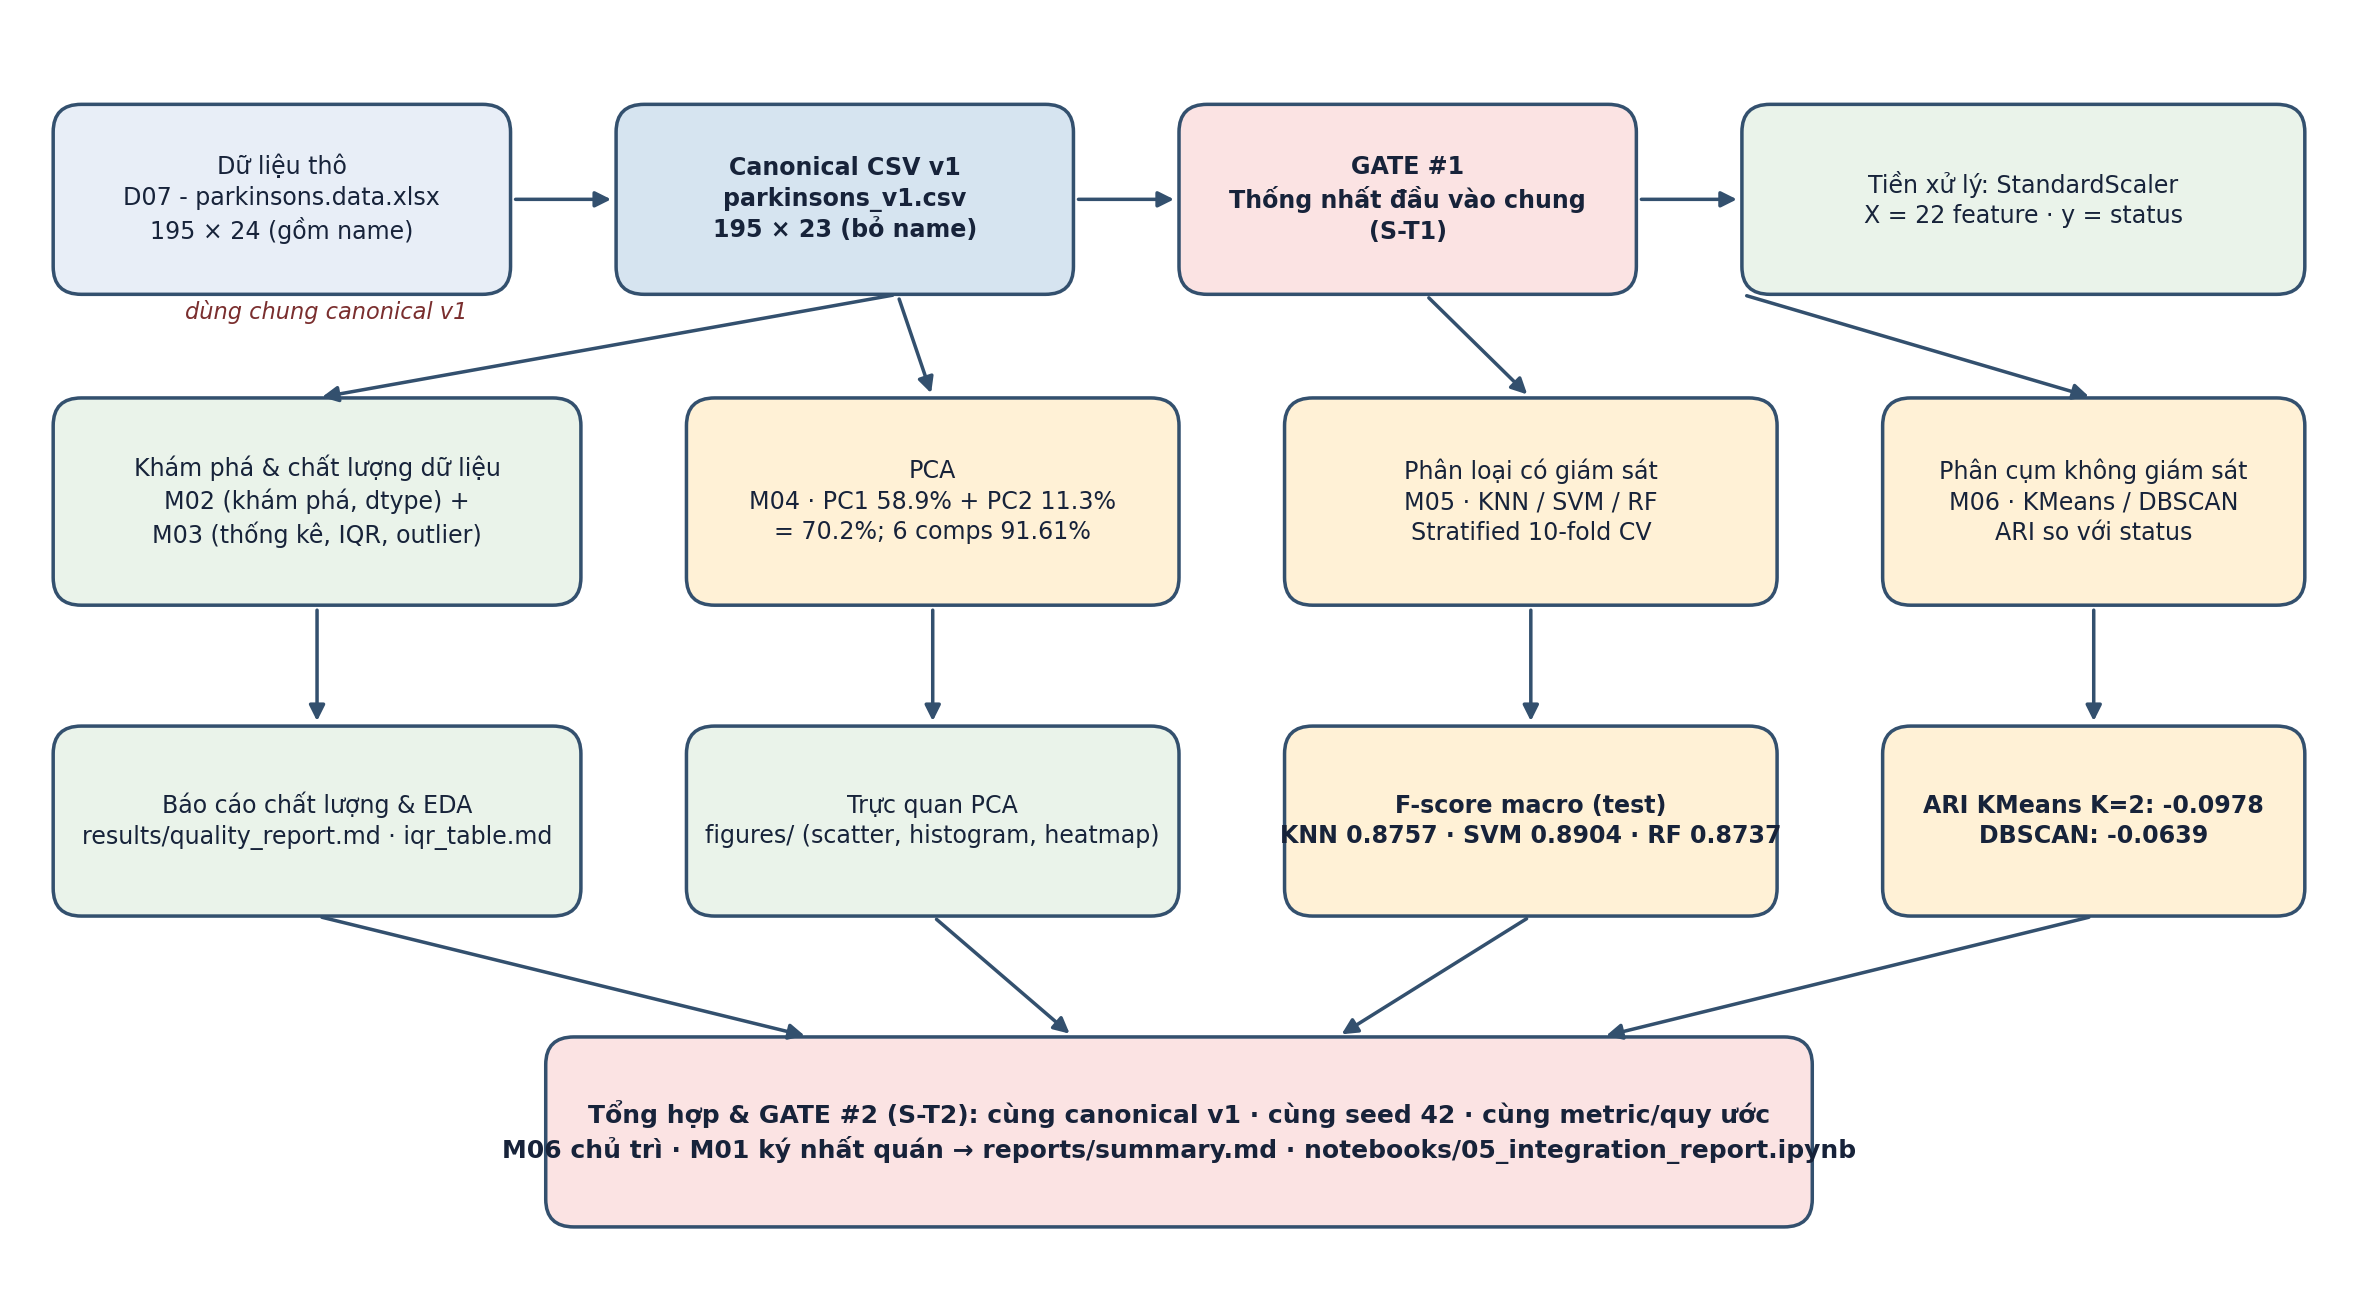
\includegraphics[width=\linewidth]{pipeline_diagram.png}
    \caption{Sơ đồ quy trình khai phá dữ liệu và các cổng kiểm soát}
    \label{fig:pipeline}
\end{figure}
\source{Tự biên soạn.}

Quy trình có hai cổng chất lượng bắt buộc:
\begin{itemize}
    \item \textbf{GATE \#1 (S-T1):} thống nhất đầu vào chuẩn \texttt{parkinsons\_v1.csv};
          các bước M02-M06 chỉ được chạy khi đầu ra của M01 đã sẵn sàng.
    \item \textbf{GATE \#2 (S-T2):} kiểm tra nhất quán toàn bộ số liệu trước khi tổng hợp,
          gồm cùng đầu vào, cùng seed, cùng độ đo và cùng quy ước.
\end{itemize}

\section{Dữ liệu và chuẩn hoá đầu vào}

\subsection{Nguồn dữ liệu}
Dữ liệu thô là tệp \texttt{D07 - parkinsons.data.xlsx} thu thập từ bộ dữ liệu Oxford
Parkinson's Disease Detection trên UCI \cite{uci_parkinsons}, gồm 195 bản ghi $\times$ 24 cột
(22 đặc trưng + nhãn \texttt{status} + cột định danh \texttt{name}). Nhóm loại bỏ cột
\texttt{name} (thông tin cá nhân) và giữ nguyên toàn bộ đặc trưng định lượng.

\subsection{Tạo bộ dữ liệu chuẩn (canonical CSV v1)}
Một tệp CSV duy nhất được sản xuất và đóng băng làm đầu vào cho mọi bước phân tích:

\begin{lstlisting}[language=Python, numbers=none]
data/processed/parkinsons_v1.csv
# 195 dong x 23 cot = 22 feature + status
# SHA-256: 55e2fed63eb74ad19a119b43ef33d92c
#          60d60f7d6751688f1cae45d38d358153
# SHA-256 tap tin tho (.xlsx):
# d5d96457a760cd06e93b1a1d1cd6380b
# 38909c2cc82121968bb51ef29f80029a
\end{lstlisting}

Việc này giúp tránh tình trạng các thành viên dùng lần lượt các phiên bản dữ liệu khác nhau
dẫn đến số liệu không thể đối chiếu. Cấu trúc đầu vào được mô tả đầy đủ trong
\texttt{data/processed/}\allowbreak\texttt{schema\_v1.md}.

\section{Kiến trúc thực hiện}

\subsection{Cấu trúc kho lưu trữ}

\begin{table}[H]
\centering
\caption{Cấu trúc chính của kho lưu trữ}
\begin{tabular}{|l|>{\raggedright\arraybackslash}p{8.6cm}|}
\hline
\textbf{Đường dẫn} & \textbf{Vai trò} \\
\hline
\texttt{data/raw/} & Dữ liệu thô và manifest nguồn \\
\hline
\texttt{data/processed/} & Canonical CSV v1 và schema \\
\hline
\texttt{notebooks/} & 5 notebook phân tích có lần lượt M01-M06 \\
\hline
\texttt{src/} & Hàm dùng chung và pipeline tổng hợp (\texttt{pipeline.py}) \\
\hline
\texttt{results/} & Báo cáo, bảng số liệu, hình ảnh, \texttt{pipeline\_summary.json} \\
\hline
\texttt{reports/} & Báo cáo tổng hợp cuối cùng \\
\hline
\texttt{workspaces/member-XX/} & Không gian làm việc của từng thành viên \\
\hline
\end{tabular}
\end{table}

\subsection{Pipeline tổng hợp}
Để kiểm chứng tính nhất quán, nhóm viết một lối chạy tổng hợp
(\texttt{python -m src.pipeline}) gọi lại các bước chuẩn bị dữ liệu, PCA và phân loại rồi
ghi kết quả vào \texttt{results/}\allowbreak\texttt{pipeline\_summary.json}. Lối chạy này không thay thế các
notebook chuyên sâu mà phục vụ đối chiếu chéo giữa các sản phẩm của nhóm.

\section{Quản lý công việc và đảm bảo chất lượng}

\subsection{Luồng Git và review}
Nhóm áp dụng luồng làm việc theo nhánh: mỗi nhiệm vụ tạo một nhánh riêng, mở pull request
(PR) về \texttt{main}, người phụ trách review bình luận và tag thành viên liên quan, chỉ
nhập nhánh sau khi có xác nhận đạt. Các PR đã merge bao gồm \#5 (khám phá), \#7 (tiền xử
lý-PCA), \#8 (phân loại), \#13 (thống kê/chất lượng), \#14 (phân cụm), \#16 (tổng hợp) và
\#17 (chốt gate). Đây là cách thức giúp mọi thay đổi đều được kiểm soát và truy vết.

\subsection{Bảng theo dõi nhiệm vụ}
Toàn bộ công việc được theo dõi trong \texttt{TASK\_BOARD.md} với 21 nhiệm vụ được mã hoá từ
M01-T1 tới S-T2. Mỗi nhiệm vụ chỉ được chuyển sang \texttt{Done} sau khi có bằng chứng đạt
review. Tại thời điểm tổng hợp, bảng ghi nhận \textbf{21/21 nhiệm vụ Done}; hai cổng GATE
\#1 và GATE \#2 đã được ký.

\subsection{Phân công và đóng góp}
Sáu thành viên phân công theo nhiệm vụ chính như Bảng \ref{tab:team_chap3}; nhóm điều phối
giữ vai trò cổng chất lượng, còn việc tổng hợp kết quả do hai thành viên M01 và M06 đồng sở
hữu để tránh phụ thuộc một người.

\begin{table}[H]
\centering
\caption{Phân công theo mô-đun và nghiệm thu}
\begin{tabular}{|c|l|l|}
\hline
\textbf{Mã} & \textbf{Họ và tên} & \textbf{Mô-đun / minh chứng nghiệm thu} \\
\hline
M01 & Đặng Hoàng Ân   & Dữ liệu, pipeline tổng hợp; ký GATE \#1, GATE \#2 \\
\hline
M02 & Lê Thiên Lộc    & M02-T1..T3; PR \#5 đạt review \\
\hline
M03 & Huỳnh Gia Hợp    & M03-T1..T3; PR \#13 đạt review \\
\hline
M04 & Trần Hoàng Thông & M04-T1..T3; PR \#7 đã merge \\
\hline
M05 & Ngô Thị Anh Thư   & M05-T1..T3; PR \#8 đạt review \\
\hline
M06 & Nguyễn Hoàng Bách & M06-T1..T3; PR \#14, PR \#16 đạt review \\
\hline
\end{tabular}
\label{tab:team_chap3}
\end{table}

\section{Môi trường thực nghiệm}

Thực nghiệm được thực hiện trên Python với các thư viện chuẩn của khoa học dữ liệu. Bảng
dưới ghi phiên bản được dùng ở lần chạy tổng hợp để cùng một cấu hình.

\begin{table}[H]
\centering
\caption{Môi trường thực nghiệm}
\begin{tabular}{|>{\raggedright\arraybackslash}p{5.2cm}|>{\raggedright\arraybackslash}p{10.2cm}|}
\hline
\textbf{Thành phần} & \textbf{Phiên bản / giá trị} \\
\hline
Python & 3.14.0 \\
\hline
numpy / pandas / scipy & 2.4.2 / 3.0.3 / 1.17.1 \\
\hline
scikit-learn & 1.9.0 \\
\hline
matplotlib / seaborn & 3.10.8 / 0.13.2 \\
\hline
Jupyter (nbformat, nbclient, nbconvert) & 5.11.1 / 0.11.0 / 7.17.2 \\
\hline
Hạt giống ngẫu nhiên & 42 \\
\hline
Kiểm định chéo & StratifiedKFold 10 (ngoài), GridSearchCV 5 (trong) \\
\hline
Độ đo chính & F-score macro (phân loại), ARI (phân cụm) \\
\hline
\end{tabular}
\end{table}

Các notebook M06 ban đầu chạy trên phiên bản thư viện khác (ví dụ scikit-learn 1.9.1);
kết quả vẫn khớp khi kiểm tra chéo, và nhóm đã ghi rõ phiên bản trong từng báo cáo để đảm
bảo minh bạch.

\section{Phương pháp đánh giá}

Với phân loại, hiệu năng được báo cáo dưới dạng trung bình $\pm$ độ lệch chuẩn của F-score
macro trên 10 fold kiểm tra, kèm F-score weighted và F-score trên tập huấn luyện để phát
hiện quá khớp. Với phân cụm, nhóm chọn số cụm K bằng silhouette, sau đó so sánh cụm với nhãn
bằng ARI; DBSCAN được chọn tham số bằng điểm uốn (knee) của khoảng cách láng giềng thứ
\texttt{min\_samples} và kiểm tra chéo trên lưới tham số. Mọi kết quả đều được ghi lại đầy
đủ trong thư mục \texttt{results/} kèm tham số, seed và phiên bản thư viện.
